% generated by paper/make_figure.py -- do not edit
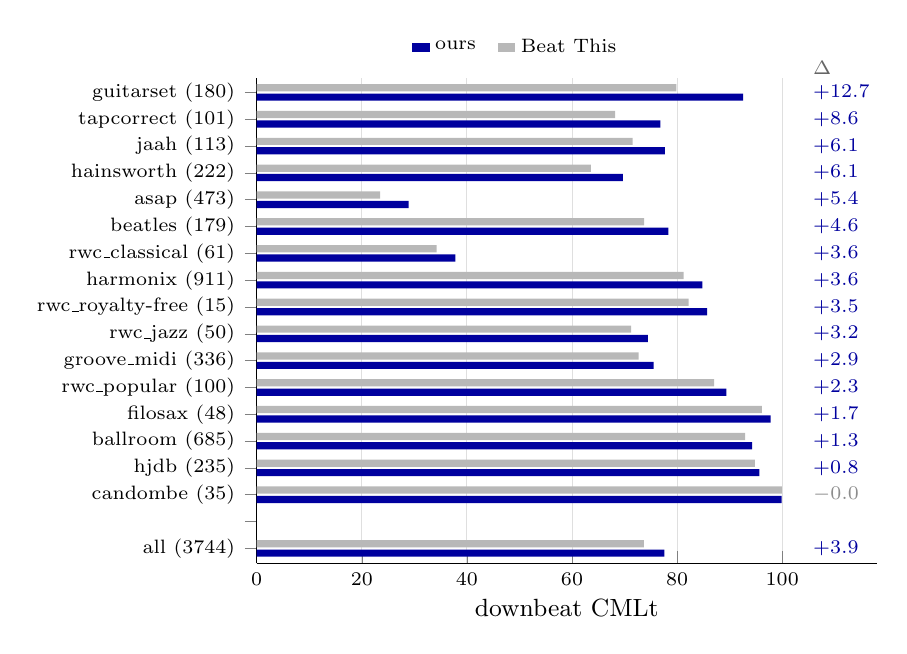
\begin{tikzpicture}
\begin{axis}[
  xbar, width=0.78\columnwidth, height=3.05in,
  bar width=2.6pt, bar shift=0pt,
  enlarge y limits={abs=0.55},
  xmin=0, xmax=118, xtick={0,20,40,60,80,100},
  ytick={0,1,2,3,4,5,6,7,8,9,10,11,12,13,14,15,16,17},
  yticklabels={{all (3744)},{},{candombe (35)},{hjdb (235)},{ballroom (685)},{filosax (48)},{rwc\_popular (100)},{groove\_midi (336)},{rwc\_jazz (50)},{rwc\_royalty-free (15)},{harmonix (911)},{rwc\_classical (61)},{beatles (179)},{asap (473)},{hainsworth (222)},{jaah (113)},{tapcorrect (101)},{guitarset (180)}},
  tick label style={font=\scriptsize},
  xlabel={downbeat CMLt}, xlabel style={font=\small, yshift=2pt},
  axis y line*=none, axis x line*=bottom,
  xmajorgrids, grid style={gray!25, line width=0.3pt},
  legend style={font=\scriptsize, draw=none, fill=none,
                 at={(0.42,1.02)}, anchor=south, legend columns=2,
                 /tikz/every even column/.append style={column sep=6pt}},
  % xbar draws two swatches per entry by default; one filled rectangle is enough
  legend image code/.code={\draw[#1, draw=none]
      (0cm,-0.055cm) rectangle (0.22cm,0.055cm);},
  clip=false,
]
\addplot[fill=blue!62!black, draw=none, bar shift=-1.7pt] coordinates {(77.58,0) (99.90,2) (95.63,3) (94.25,4) (97.80,5) (89.35,6) (75.53,7) (74.42,8) (85.72,9) (84.78,10) (37.82,11) (78.33,12) (28.92,13) (69.66,14) (77.65,15) (76.82,16) (92.57,17)};
\addplot[fill=black!28, draw=none, bar shift=1.7pt] coordinates {(73.67,0) (99.92,2) (94.80,3) (92.95,4) (96.11,5) (87.06,6) (72.66,7) (71.26,8) (82.19,9) (81.22,10) (34.24,11) (73.74,12) (23.50,13) (63.61,14) (71.53,15) (68.21,16) (79.84,17)};
\legend{ours, Beat This}
\node[anchor=west, font=\scriptsize, text=blue!62!black] at (axis cs:104,0) {$+3.9$};
\node[anchor=west, font=\scriptsize, text=black!45] at (axis cs:104,2) {$-0.0$};
\node[anchor=west, font=\scriptsize, text=blue!62!black] at (axis cs:104,3) {$+0.8$};
\node[anchor=west, font=\scriptsize, text=blue!62!black] at (axis cs:104,4) {$+1.3$};
\node[anchor=west, font=\scriptsize, text=blue!62!black] at (axis cs:104,5) {$+1.7$};
\node[anchor=west, font=\scriptsize, text=blue!62!black] at (axis cs:104,6) {$+2.3$};
\node[anchor=west, font=\scriptsize, text=blue!62!black] at (axis cs:104,7) {$+2.9$};
\node[anchor=west, font=\scriptsize, text=blue!62!black] at (axis cs:104,8) {$+3.2$};
\node[anchor=west, font=\scriptsize, text=blue!62!black] at (axis cs:104,9) {$+3.5$};
\node[anchor=west, font=\scriptsize, text=blue!62!black] at (axis cs:104,10) {$+3.6$};
\node[anchor=west, font=\scriptsize, text=blue!62!black] at (axis cs:104,11) {$+3.6$};
\node[anchor=west, font=\scriptsize, text=blue!62!black] at (axis cs:104,12) {$+4.6$};
\node[anchor=west, font=\scriptsize, text=blue!62!black] at (axis cs:104,13) {$+5.4$};
\node[anchor=west, font=\scriptsize, text=blue!62!black] at (axis cs:104,14) {$+6.1$};
\node[anchor=west, font=\scriptsize, text=blue!62!black] at (axis cs:104,15) {$+6.1$};
\node[anchor=west, font=\scriptsize, text=blue!62!black] at (axis cs:104,16) {$+8.6$};
\node[anchor=west, font=\scriptsize, text=blue!62!black] at (axis cs:104,17) {$+12.7$};
\node[anchor=west, font=\scriptsize, text=black!60] at (axis cs:104,17.9) {$\Delta$};
\end{axis}
\end{tikzpicture}
